% !TEX root = thesis.tex
% ===============================================
% ===============================================
% 	LaTeX Chapter File - Main Text
% ===============================================
% ===============================================
\chapter{Latex syntax examples}

\textcolor{red}{This chapter must be removed in the final version to be printed.}

\section{Test acronyms}

first time \gls{fpga} and \gls{noc}. Second time \gls{fpga} and \gls{noc}.


\section{Test figures}

Here are some examples on how to place figures. \Cref{fig:tiefpass} is just a single figure.

\begin{figure}[htb]
	\centering
	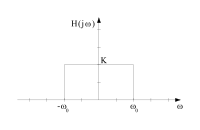
\includegraphics[width=.5\linewidth]{figures/tiefpass.png}
	\caption{Idealer Tiefpass}
	\label{fig:tiefpass}
\end{figure}

But \cref{fig:functions} is one figure-environment with two figures. You can reference to each of the figures in the environment. \Cref{fig:si-function} is a Si-function and \cref{fig:dreieck} is a triangular function.

\begin{figure}[htb]
	\centering
	\begin{subfigure}[b]{0.4\textwidth}
		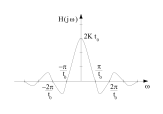
\includegraphics[width=\textwidth]{figures/Si-function.png}
		\caption{Si-Funktion}
		\label{fig:si-function}
	\end{subfigure}
	~ %add desired spacing between images, e. g. ~, \quad, \qquad, \hfill etc. 
	%(or a blank line to force the subfigure onto a new line)
	\begin{subfigure}[b]{0.4\textwidth}
		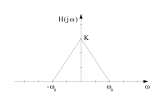
\includegraphics[width=\textwidth]{figures/dreieck.png}
		\caption{Dreieck}
		\label{fig:dreieck}
	\end{subfigure}
	\caption{Pictures of functions}
	\label{fig:functions}
\end{figure}

Figures are always placed \emph{after} referencing them.

\section{Test tables}

This is an example of a simple table. \Cref{tab:flocklab_clock_offset} shows random stuff.
%
\begin{table}[htb]
	\centering
	\caption{A simple table.}
	\begin{tabular}{l c c}
		\toprule
		Node id & DCO frequency & DCO offset\\ \midrule
		11, 17, 23 & 4,131,389 Hz & -1.5\% \\
		4, 10, 16, 22, 28 & 4,152,361 Hz & -1\% \\
		1, 3, 7, 13, 15, 19, 25, 27, 33 & 4,194,304 Hz & 0\% \\
		6, 18, 24 & 4,236,247 Hz & +1\% \\
		2, 8, 14, 20, 26, 32 & 4,257,218 Hz & +1.5\% \\
		\bottomrule
	\end{tabular}
	\label{tab:flocklab_clock_offset}
\end{table}

As figures, tables should be places \emph{after} referencing them.

\section{Test citation}

\cite{Goehringer2013}, \cite{Logvinenko2014}, \cite{Ogras2013}, \cite{Rantala2006}


\cite{Adetomi2018}
\cite{Adomat1996}
\cite{Andrews2005}
\cite{Arora2021}
\cite{Bansal2006}
\cite{Bloom}
\cite{Cashmore2015}
\cite{Chapin1996}
\cite{Chen2016}
\cite{Chervenak1999}
\cite{Conficconi2021}
\cite{Dally2001}
\cite{Djordjevic1996}
\cite{Fernandes2011}
\cite{Fernando2010}
\cite{Ferrandi2006}
\cite{Fowers2018}
\cite{FuYao2017}
\cite{Gandhi2005}
\cite{Golson1994}
\cite{greenwade93}
\cite{GuoKaiyuan2018}
\cite{GuoLicheng2022}
\cite{Hennessy2019}
\cite{Ibarra1977}
\cite{JiangYingtao2004}
\cite{JinShiyuan2008}
\cite{Kalms2019}
\cite{Koch2021}
\cite{Langhammer2021}
\cite{Leuenberger2021}
\cite{Mathwork}
\cite{Miyauchi2020}
\cite{Mohan2021}
\cite{Montanno2010}
\cite{Nikolic2021}
\cite{Nowatzki}
\cite{Oh1999}
\cite{Petersen2021}
\cite{Podlubne2018}
\cite{Podlubne2021}
\cite{Pravin18}
\cite{quigley2009ros}
\cite{Rainey}
\cite{Reggiani2021}
\cite{Ritschel2019}
\cite{Saez1999}
\cite{Scheduling_Handbook}
\cite{Schmit}
\cite{Stallings2008}
\cite{TangYi2015}
\cite{Thapliyal2010}
\cite{Trimberger}
\cite{Vasile2014}
\cite{Witte2018}
\cite{Wulf2020}
\cite{YangMing2018}
\cite{Zagan2019}
\cite{Zagan2020}
\cite{ZhaYue2021}
